\documentclass[10pt,twocolumn]{article}

\usepackage[margin=0.72in]{geometry}
\usepackage[T1]{fontenc}
\usepackage{lmodern}
\usepackage{microtype}
\usepackage{float}
\usepackage{pgfplots}
\pgfplotsset{compat=1.18}

\title{UNO-UMB: Uncertainty-Aware Cell Sleep Control for QoS-Safe RAN Energy Savings}
\author{Haoyu}
\date{}

\raggedbottom

\begin{document}
\maketitle

\begin{abstract}
Cell sleep can reduce radio access network energy use, but load shifts can turn
apparently safe sleep decisions into quality-of-service violations.  This paper
presents UNO-UMB, an ns-3 prototype for uncertainty-aware cell sleep control.
UNO-UMB combines a lightweight digital-twin risk gate, a latent-demand wakeup
rule for unannounced shifts, and a forecast-risk margin that can be selectively
inflated for tight close-offload decisions.  In an expanded LTE evaluation over
three seeds, two runs, and three inter-site spacings, the adaptive wakeup
recovers all 18/18 feasible center-burst rows where static risk gating is safe
on 14/18.  On a right-edge transition surface with a 25\% underpredicted
forecast, the forecast margin recovers all 16/16 feasible rows with 16.744\%
mean safe energy saving, while a stronger global margin lowers safe saving and
leaves one feasible row unsafe.  These preliminary results suggest
that spatially conditioned uncertainty control can preserve energy savings
while bounding transition risk.
\end{abstract}

\section{Introduction}

Radio access networks are increasingly energy constrained: base stations are
dimensioned for busy periods, but much of the deployment may be lightly loaded
for long intervals.  Cell sleep is a direct way to reduce active energy, yet a
sleep decision changes the load and radio geometry seen by neighboring cells.
The central difficulty is therefore not only to find idle cells, but to decide
which apparently idle cells can sleep without creating a quality-of-service
violation after traffic shifts.

UNO-UMB studies this problem in ns-3.  The current prototype focuses on a
simple but paper-relevant question: can a lightweight uncertainty-aware
controller recover energy savings while avoiding controller-induced failures in
workloads that remain feasible when all cells stay active?

The contributions are:

\begin{itemize}
\item A digital-twin cell sleep controller that evaluates candidate sleep
decisions against per-UE offered load and predicted active-cell utilization.
\item A latent-demand wakeup mechanism that reacts to unannounced load shifts
by reactivating sleeping preferred cells when doing so would relieve active
cell stress.
\item A forecast-risk margin with selective overlap inflation, which applies a
stronger bound only when a tight utilization decision also uses close offload
geometry.
\item A feasible-row evaluation method that separates controller-induced
violations from offered-load overload by comparing every controller row against
the matching all-on reference row.
\end{itemize}

\section{Controller Design}

UNO-UMB operates as a periodic cell sleep controller with event-triggered
reevaluation when demand changes.  For each candidate cell, the controller
estimates whether sleeping the cell would overload the remaining active cells.
The baseline twin policy keeps a cell active when the estimated risk exceeds a
configured guard.

The adaptive controller adds a latent-demand wakeup gate.  When a sleeping cell
is the preferred serving cell for enough offered demand, and waking it would
reduce peak active-cell utilization by a configured relief threshold, the
controller reactivates that cell.  This mechanism targets unannounced load
shifts where a previously safe sleep decision becomes unsafe before the next
steady-state placement.

For anticipated traffic shifts, UNO-UMB supports a lead-time forecast gate.  A
forecast can carry both a magnitude error and an uncertainty margin.  The
selective overlap variant uses a base uncertainty margin for ordinary forecast
decisions, then inflates the margin only when the candidate decision has small
utilization slack and nearby offload geometry.  This keeps the base margin on
placements where it is already sufficient and avoids charging a stronger global
margin to every forecasted decision.

\section{Evaluation Setup}

The prototype is implemented as an ns-3 contribution module and evaluated using
an LTE cell sleep example.  Unless otherwise noted, the main rows use 16 UEs, a
1.0 Mb/s per-UE base offered load, a 12 s simulation, and a burst window from
3 s to 10 s.  The expanded controller table uses ideal LTE RRC signaling to
avoid treating stressed over-the-air control-plane scheduler assertions as
cell-sleep controller outcomes.

The evaluation reports three classes of outcome.  First, the all-on reference
identifies whether the offered-load scenario is feasible without cell sleep.
Second, controller rows are counted only when the matching all-on row is
feasible.  Third, safe energy saving is measured only for controller rows that
avoid induced violations.

\section{Results}

Figure~\ref{fig:evaluation-tradeoff} plots the two main mechanisms as
feasible-row safety versus safe energy saving.  The center-burst panel shows
the adaptive wakeup trading energy saving for complete safety on the feasible
surface.  The right-edge panel shows a different pattern: the forecast margin
moves the controller to the upper-right safety frontier, while the stronger
global margin is both less safe and less energy efficient on the expanded
surface.

\begin{figure}[H]
\centering
% Generated from paper/data/main-evaluation-summary.csv by utils/uno-umb-paper-figures.py.
\begin{minipage}{0.98\linewidth}
\centering
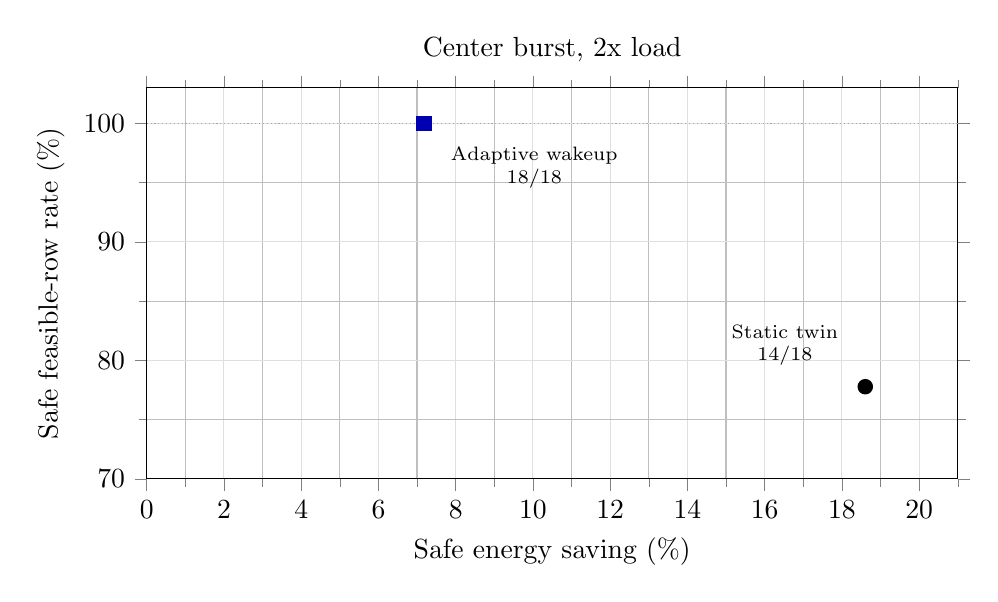
\begin{tikzpicture}
\begin{axis}[
  title={Center burst, 2x load},
  width=0.98\linewidth,
  height=0.54\linewidth,
  xmin=0,
  xmax=21,
  ymin=70,
  ymax=103,
  xlabel={Safe energy saving (\%)},
  ylabel={Safe feasible-row rate (\%)},
  grid=both,
  major grid style={draw=gray!25},
  minor tick num=1,
  tick align=outside,
  clip=false,
]
  \addplot[densely dotted, gray!70] coordinates {(0,100) (21,100)};
  \addplot[only marks, mark=*, mark size=2.6pt, color=black, mark options={fill=black}] coordinates {(18.604,77.778)};
  \node[font=\scriptsize, align=center, anchor=south east] at (axis cs:18.154,78.778) {Static twin\\14/18};
  \addplot[only marks, mark=square*, mark size=2.6pt, color=blue!70!black, mark options={fill=blue!70!black}] coordinates {(7.176,100.000)};
  \node[font=\scriptsize, align=center, anchor=north west] at (axis cs:7.626,98.800) {Adaptive wakeup\\18/18};
\end{axis}
\end{tikzpicture}
\end{minipage}
\par\vspace{0.8ex}
\begin{minipage}{0.98\linewidth}
\centering
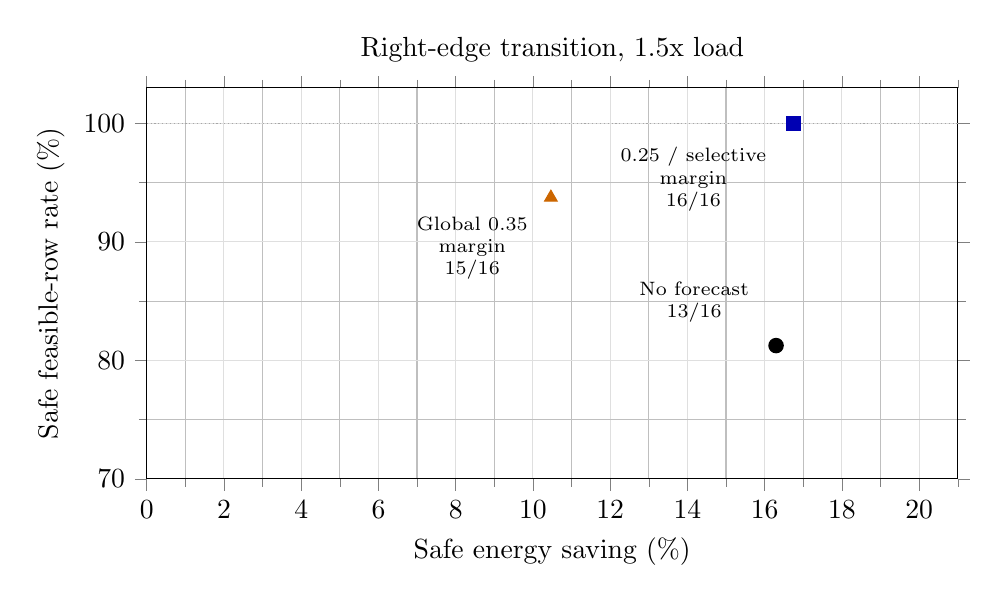
\begin{tikzpicture}
\begin{axis}[
  title={Right-edge transition, 1.5x load},
  width=0.98\linewidth,
  height=0.54\linewidth,
  xmin=0,
  xmax=21,
  ymin=70,
  ymax=103,
  xlabel={Safe energy saving (\%)},
  ylabel={Safe feasible-row rate (\%)},
  grid=both,
  major grid style={draw=gray!25},
  minor tick num=1,
  tick align=outside,
  clip=false,
]
  \addplot[densely dotted, gray!70] coordinates {(0,100) (21,100)};
  \addplot[only marks, mark=*, mark size=2.6pt, color=black, mark options={fill=black}] coordinates {(16.295,81.250)};
  \node[font=\scriptsize, align=center, anchor=south east] at (axis cs:15.845,82.350) {No forecast\\13/16};
  \addplot[only marks, mark=square*, mark size=2.6pt, color=blue!70!black, mark options={fill=blue!70!black}] coordinates {(16.744,100.000)};
  \node[font=\scriptsize, align=center, anchor=north east] at (axis cs:16.294,98.800) {0.25 / selective\\margin\\16/16};
  \addplot[only marks, mark=triangle*, mark size=2.6pt, color=orange!80!black, mark options={fill=orange!80!black}] coordinates {(10.465,93.750)};
  \node[font=\scriptsize, align=center, anchor=north east] at (axis cs:10.115,92.950) {Global 0.35\\margin\\15/16};
\end{axis}
\end{tikzpicture}
\end{minipage}

\caption{Safety-energy tradeoff on the expanded ideal-RRC evaluation.  Points
report the safe feasible-row rate and mean safe energy saving; labels give safe
rows over feasible controller rows.}
\label{fig:evaluation-tradeoff}
\end{figure}

Table~\ref{tab:center} summarizes the expanded center-burst rows at 2x offered
load.  Static twin control is safe on 14/18 feasible rows.  Adaptive twin
control removes the induced violations by waking cells earlier, at the cost of
lower energy saving.

\begin{table}[H]
\centering
\caption{Expanded center-burst 2x feasible-row results.}
\label{tab:center}
\begin{tabular}{llll}
\hline
Scenario & Policy & Safe rate & Saving \\
\hline
2.0x & twin & 14/18 & 18.604\% \\
2.0x & adaptive & 18/18 & 7.176\% \\
\hline
\end{tabular}
\end{table}

Table~\ref{tab:right-edge} summarizes the right-edge transition surface across
475 m, 500 m, and 525 m spacing.  The no-forecast controllers leave feasible
rows unsafe.  The base 0.25 margin and selective overlap margin both recover
all 16 feasible rows.  A global 0.35 margin is more conservative, but loses one
feasible row and substantially lowers safe energy saving.

\begin{table}[H]
\centering
\caption{Expanded right-edge 1.5x transition surface.}
\label{tab:right-edge}
\begin{tabular}{llll}
\hline
Control & Policy & Safe rate & Saving \\
\hline
No forecast & twin & 13/16 & 16.295\% \\
No forecast & adaptive & 12/16 & 10.614\% \\
0.25 margin & twin & 16/16 & 16.744\% \\
0.25 margin & adaptive & 16/16 & 16.744\% \\
0.35 margin & twin & 15/16 & 10.465\% \\
0.35 margin & adaptive & 15/16 & 10.465\% \\
Selective margin & twin & 16/16 & 16.744\% \\
Selective margin & adaptive & 16/16 & 16.744\% \\
\hline
\end{tabular}
\end{table}

The forecast-margin result is the strongest current evidence for the paper.  It
removes every induced right-edge transition violation in the expanded feasible
surface while slightly increasing safe mean energy saving relative to
no-forecast control, because unsafe high-saving rows no longer have to be
discarded from the safe set.  Selective overlap inflation preserves this result
without paying the energy and residual safety cost of the global 0.35 margin.

\section{Discussion and Limitations}

The present results are intentionally framed as feasible-row results, not as a
claim that every offered-load scenario can be made safe by control.  Some rows
are overloaded even when all cells remain active, and those rows are excluded
from controller safety rates.

The next validation step is a larger replicated sweep over more seeds, UE
rates, UE counts, and spacings.  The prototype should also be compared against
stronger baselines, including controllers with calibrated static margins and
controllers that use forecast lead time without spatially selective inflation.

\section{Related Work}

This section will be filled with the final venue-specific literature review.
The key groups to cover are RAN energy saving and cell sleep, digital-twin or
model-predictive radio control, uncertainty-aware resource management, and
robust handover or load-balancing methods.

\section{Conclusion}

UNO-UMB shows that cell sleep safety can benefit from separating reactive and
forecasted uncertainty.  Latent-demand wakeup protects feasible unannounced
center bursts, while selective overlap-gated forecast margins protect hard
right-edge transitions without imposing a global conservative energy cost.  The
current ns-3 prototype and experiment notes are ready for a first manuscript
draft and a broader replication sweep.

\end{document}
